% Meta Setting
\documentclass[10pt]{article}

% Formatting packages below.
\usepackage[left=1in,right=1in,top=1in,bottom=1in]{geometry}
\usepackage{float}
\usepackage{booktabs}
\usepackage{caption}
\usepackage{subcaption}
\usepackage{graphicx}

\usepackage{Sweave}
\begin{document}
\Sconcordance{concordance:group4_draft_4.tex:group4_draft_4.Rnw:%
1 11 1 1 0 8 1 1 21 11 1 1 17 1 2 4 1 1 7 1 2 10 1 1 102 9 0 1 2 10 1 1 %
40 1 2 10 1 1 115 8 0 1 2 4 1 1 60 8 0 1 2 7 1 1 67 1 2 2 1}

\title{Interpreting The Effect Of COVID On Motor Vehicle Accidents in the New York Metropolitan Area (SQL Integration)}
\author{Jian Ruan, Zach Yu, Carrie Hashimoto, Sophia Lyu (Undergraduate), Patrick Yee (Graduate)}
\maketitle

% Install packages & Setup Libraries

%-----------------------------------------------------------------------
\section{Introduction}
COVID-19 quarantine limited people to remote work and in-home activities. It's likely that the COVID-19 restriction of transportation decreased the number of car crashes in NYC. To test out our hypothesis, we first compare and contrast the car crash distribution through geographical mapping, and later through time-series analysis and free-text analysis based on New York Times articles. 

For this report, we transferred our data to SQL database to significantly reduce the size of the data.frames and increase the efficiency of data analysis. 

%-----------------------------------------------------------------------
\section{Geographical Distribution}
\begin{figure}[H]
\centering
% Jian Code - GIS Plot
\includegraphics{group4_draft_4-002}
\caption{Accidents Distribution Before COVID.}
\end{figure}

\begin{figure}[H]
\centering
\includegraphics{group4_draft_4-003}
\caption{Accidents Distribution After COVID.}
\end{figure}

Each incident is mapped as a blue dot (x = lattitude,y = longitude) based on the OpenStreetMap API for New York City. The bluer the area shows, the more accidents happened. \\
\noindent
As shown in Figure 1, there is a sudden decrease in the number of accidents coinciding with the start of the COVID-19 pandemic, especially around the two most populous areas - Manhattan and Brooklyn. Since COVID transmitted quickly among large group of population, Manhattan and Brooklyn were the top two areas with people tested positive at the start of 2020. As a result, the quarantine policy for Manhattan and Brooklyn was more strict than other places, and people adapted to online activities to avoid infection.
%-----------------------------------------------------------------------
\section{Contributing Factors}
\begin{figure}[H]
\centering
% Carrie Code - Time Series.
\begin{Schunk}
\begin{Soutput}
<SQLiteResult>
  SQL  
DROP VIEW tableCrashesSubset

  ROWS Fetched: 0 [complete]
       Changed: 0
\end{Soutput}
\end{Schunk}
\caption{Contributing Factors Line Plot.}
\end{figure}

We had previously created pie plots of the yearly relative frequency of the ten most common contributing factors to car crashes. However, these plots were difficult to interpret because some of the changes between fractions by year were fairly subtle and the color gradients aren’t the most pronounced. We decided to visualize something similar using a different type of plot for this draft. \\
\noindent
Interpretation: This line plot shows the relative frequency of crashes caused by each of the ten contributing factors that cause the most injuries by year. Ranking by the contributing factors that cause the most injuries was a way of ensuring that we considered the most relevant causes, and using a line plot allows us to look at the changes in proportion of each factor over time in addition to the importance of each factor relative to the others.

%-----------------------------------------------------------------------
\begin{figure}[H]
\centering
% Zach Code - Bar Plot.
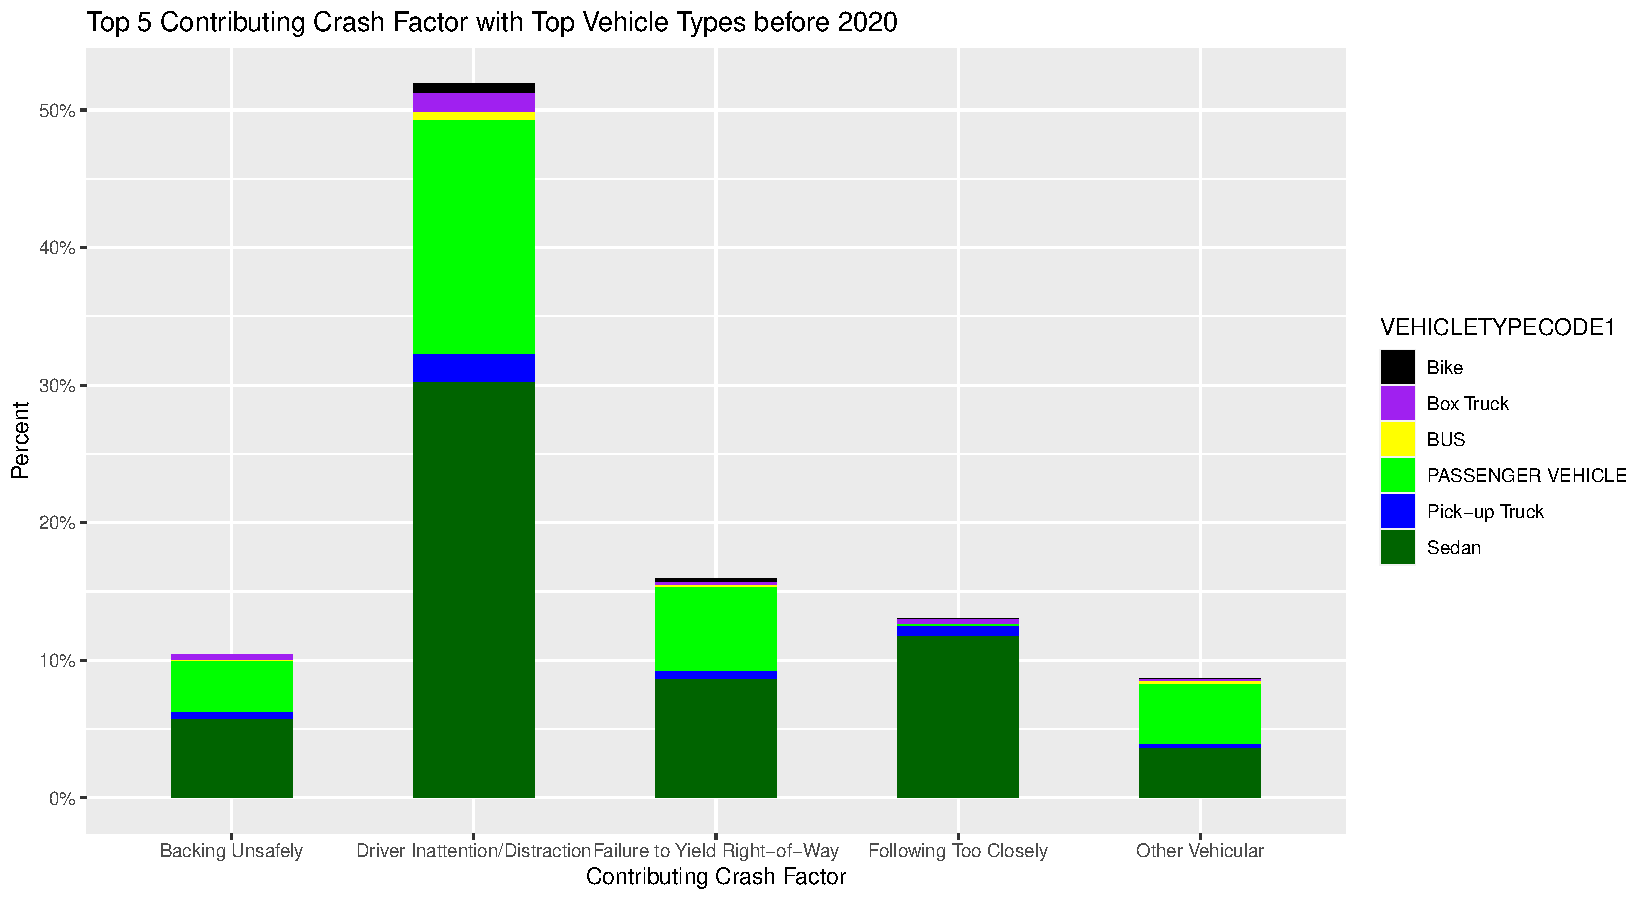
\includegraphics{group4_draft_4-005}
\caption{Barplot of contributing factors, accounting for vehicle type}
\end{figure}
It was taken into consideration what were the top contributing factors for New York crashes (excluding the unspecified causes). Many crash factors were accounted for so the top 5 contributing factors (excluding unspecified) were examined. Within the data of top 5 contributing crash factors, the proportion of vehicle type involved was implemented by color. Below is the bar graph of the percentage of crashes occurring with the top 5 crash factors and the type of vehicle taken into account.\\
\noindent
The bar graph shows that driver inattention/ distraction accounts significantly for the proportion of crashes in New York city. In addition, within each of the top 5 crash factors, sedan accounts for the most number of crashes, supporting the fact that sedan is involved in the most amount of crashes. We can further explore these high-risk contributing factors by visualizing raw relative counts. An array of pie charts show the relative frequency of each of the top ten contributing factors to car crashes by borough and number of fatalities. Feature engineering was performed to combine related contributing factors into new categories such as ”Fatigued/drowsy/sleepy/unconscious,” and entries with unknown borough were dropped.

%-----------------------------------------------------------------------
\section{Time Series Analysis}
\begin{figure}[H]
\centering
% Patrick Code - NYT analysis.
\begin{Schunk}
\begin{Soutput}
<SQLiteResult>
  SQL  DROP VIEW IF EXISTS propMentions
  ROWS Fetched: 0 [complete]
       Changed: 0
\end{Soutput}
\end{Schunk}
\includegraphics{group4_draft_4-006}
\caption{Regression Plot}
\end{figure}

\begin{figure}[H]
\centering
\begin{Schunk}
\begin{Soutput}
<SQLiteResult>
  SQL  DROP VIEW IF EXISTS crashesMinMaxAvg
  ROWS Fetched: 0 [complete]
       Changed: 0
\end{Soutput}
\end{Schunk}
\includegraphics{group4_draft_4-007}
\caption{Ribbon Plot}
\end{figure}

%-----------------------------------------------------------------------
\section{Radar Analysis}
\begin{figure}[H]
\centering
% Sohpie Code - Radar Plot.
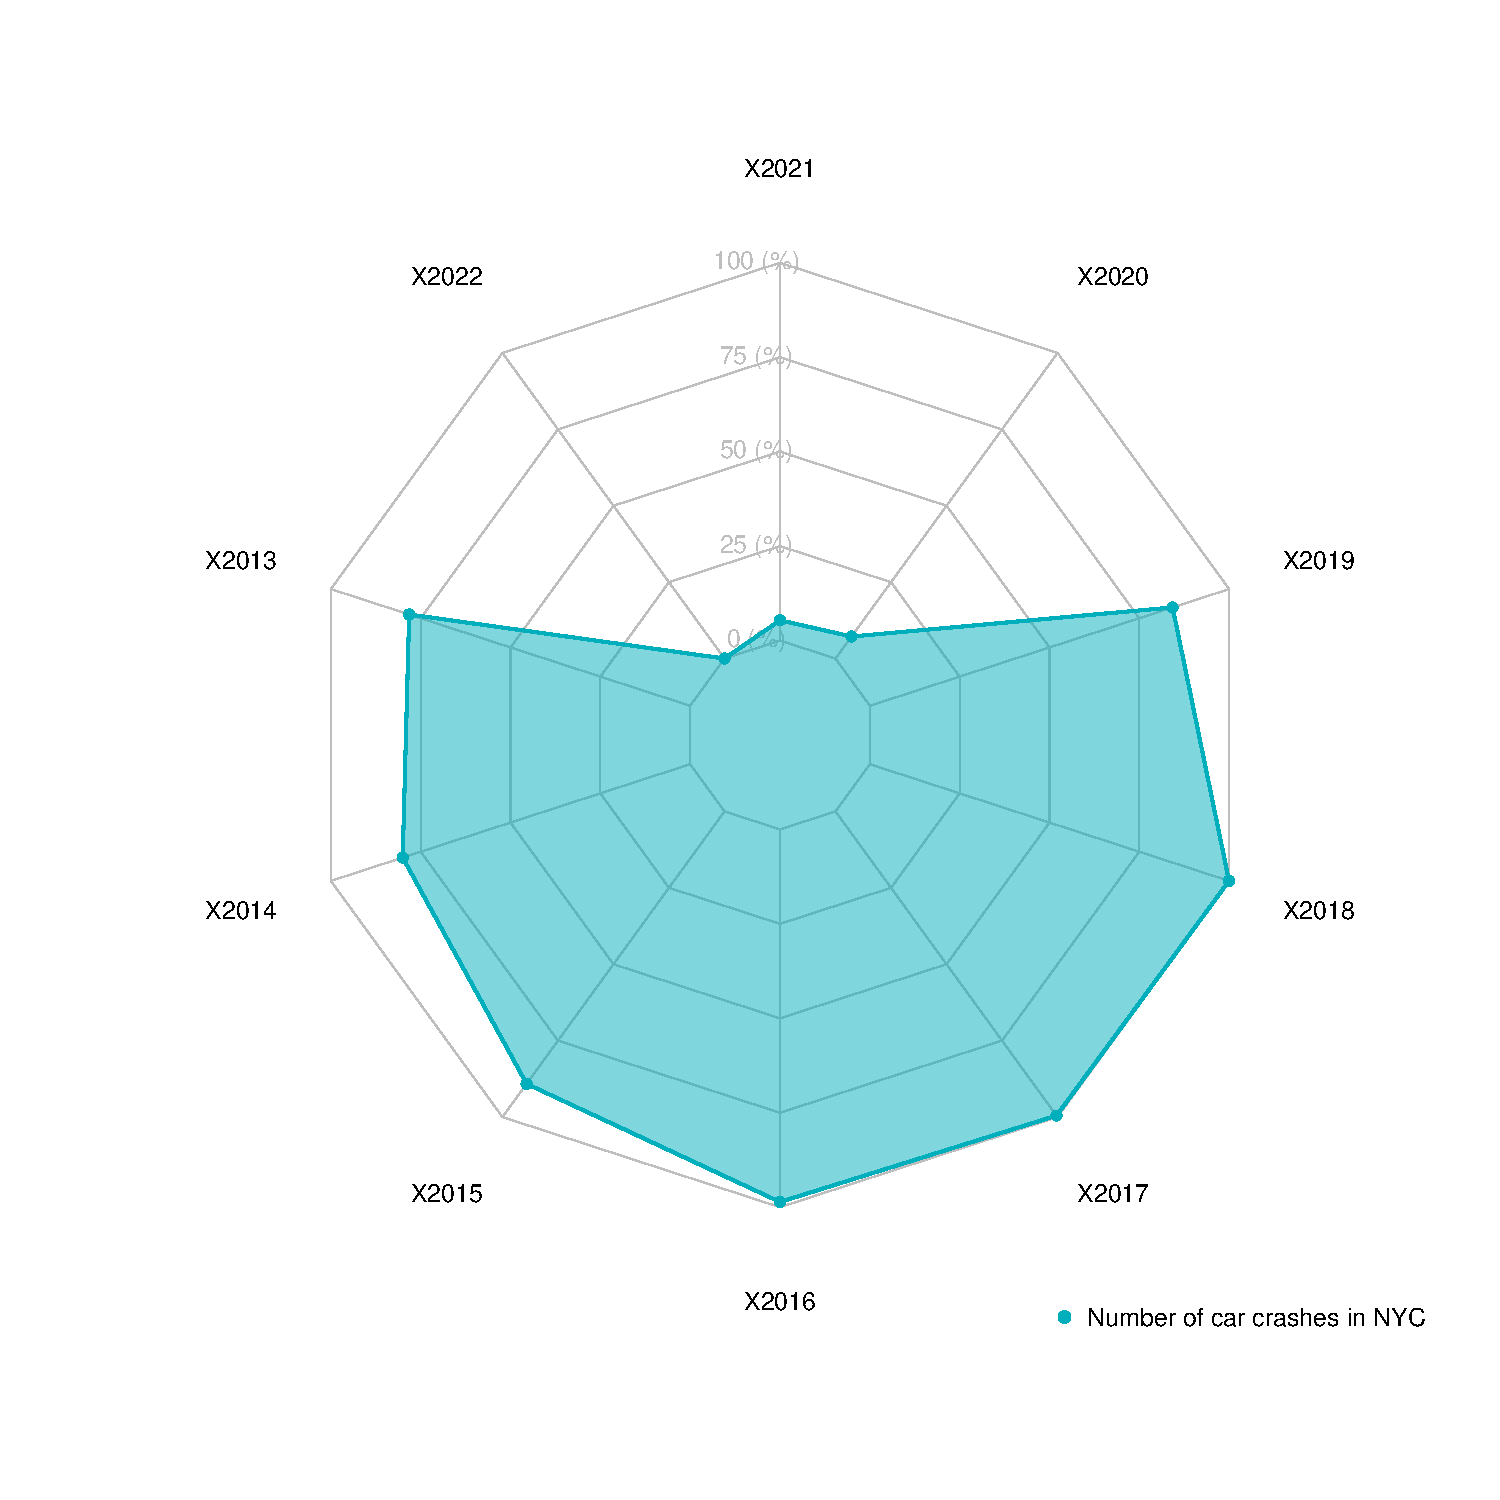
\includegraphics{group4_draft_4-008}
\caption{Radar Plot}
\end{figure}

\end{document}


